\section{直线、线段}

\subsection{直线的表示方法}
\begin{frame}
\frametitle{斜截式和两点/向量式}
\pause
直线的存储有多种方式。\newline \newline

\pause
一种是利用直线的斜截式方程y=kx+b。

这种表达方式方便判断直线的平行、求直线的交点、判断点与直线的位置关系都非常方便。但是它不能表示一条竖线，所以会受到很多的限制。\newline \newline

\pause
另一种是最常用的方法，直接存储直线上任意两个不同点的坐标$(a(x_1,y_1 ),b(x_2,y_2))$。

因为两点确定一条直线。同时，直线上的任意一个点都可以表示为$a+ \lambda (b-a)$的形式。
\end{frame}

\begin{frame}
\frametitle{一般式}
\pause
还有一种是直线的一般式$Ax+By+C=0$，它是唯一一个没有限制的直线方程，不需要考虑斜率为0、斜率为$\infty$等情况。

特别地，知道直线上两个不同的点$a,b$之后可以快速求得直线的一般式$A=y_b-y_a,B=x_b-x_a,C=x_ay_b-x_by_a$

\pause
通过直线的一般式$Ax+By+C=0$也可以快速得到直线上的两个点。

令$T=A^2+B^2$，则
\begin{displaymath}
x_1=-C*A/T,x_2=x_1+B
\end{displaymath}
\begin{displaymath}
y_1=-C*B/T,y_2=y_1-A
\end{displaymath}
\end{frame}

\subsection{直线求交}
\begin{frame}
\frametitle{向量法}
\pause
如果是两点式存储直线，那么就需要用到叉积来求交点。

\pause
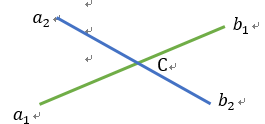
\includegraphics[width=3cm]{geometry/line.png}

\pause
$\Delta a_1 a_2 b_2$和$\Delta b_1 a_2 b_2$是同底三角形，面积之比就等于高之比。

根据平行线分线段成比例定理。这个比值也等于$|a_1 C|:|b_1 C|$

所以，我们可以得到C坐标的表达式。

\pause
\begin{displaymath}
a_1+(b_1-a_1)\frac{(S_{\Delta} a_1 a_2 b_2)}{(S_{\Delta} a_1 a_2 b_2+S_{\Delta} b_1 a_2 b_2)}
\end{displaymath}
\begin{displaymath}
=a_1+(b_1-a_1)\frac{(a_1-a_2)\times(b_2-a_2)}{(a_1-a_2 )\times(b_2-a_2 )+(b_2-a_2)\times(b_1-a_2)}
\end{displaymath}

\end{frame}

\begin{frame}
\frametitle{解析法}
\pause
如果用的是斜截式$y=k_1x+b_1,y=k_2x+b_2$(前提是斜率不为$\infty$)。

\pause
如果k,b都相同则无限交点

如果k相同b不相同则无交点

否则交点的横坐标为$-(b_1-b_2)/(k_1-k_2)$，再带入即可求出纵坐标

\pause
如果用的是一般式$A_1x+B_1y+C_1,A_2x+B_2y+C_2$

\pause
令$S=A_1B_2-A_2B_1,X=C_1B_2-C_2B_1,Y=A_1C_2-A_2C_1$

若$S=0$
	
\ \ \ \ 若$X=Y=0$，则无限交点

\ \ \ \ 否则无交点

否则$x_P=X/S,y_P=Y/S$
\end{frame}

\subsection{判点在线段上}
\begin{frame}
\pause
要判断点k是否在线段AB上，首先要判断k是否在直线AB上。

\pause
直接判$(k-A)$和$(B-A)$的叉积是否为0.

然后还要要求k位于AB之间，即$(A-k) \cdot (B-k) \le 0$
\end{frame}

\subsection{点到直线的投影}
\begin{frame}
\pause
现在要求T在直线AB上的投影

\pause
首先可以用点积求出投影离A的距离$d=\frac{ (B-A) \cdot (T-A) }{ |AB| }$

\pause
然后交点的位置即为$A+(B-A)*\frac{d}{|AB|}$

\pause
注意到点积计算的是有向距离，所以投影不在线段AB上的情况也没问题。
\end{frame}

\subsection{点到线段的最近点}
\begin{frame}
\pause
要求T到线段AB的最近点。分两种情况讨论。

\pause
如果T在直线AB上的投影在线段AB上\footnote{用点积快速判定}，则最近点为投影点。

\pause
否则最近点为A和B中的一个。
\end{frame}

\subsection{两条线段的最近距离}
\begin{frame}
\pause
如果两条线段AB和CD相交，那么距离为0。

否则距离为$\min(A$到$CD$距离，$B$到$CD$距离，$C$到$AB$距离，$D$到$AB$距离$)$ \newline \newline

\pause
证明可以分情况讨论

\pause
如果AB和CD是平行的，那么显然是正确的

\pause
否则我们考虑直线AB和直线CD的交点T。

\pause
如果T既在AB上又在CD上，则直接取T为答案，距离为0。

如果T只在AB上，那么我们会选择C和D中距离T最近的那一个。

如果T既不在AB上也不在CD上，则我们会取AB中距离T最近的一个和CD中距离T最近的那一个。
\end{frame}
